\chapter{The Library}

\section{Description}
\par
In brief \gnutls{} can be described as a portable library which offers
an API to access secure communication protocols. These protocols provide
privacy over insecure lines, and were designed to prevent 
eavesdropping, tampering, or message forgery.

\par
Technically \gnutls{} is a library which implements the \tlsI{} and 
\sslIII{} protocols. \tls{} stands for 'Transport Layer Security' and is the sucessor of \ssl{}, 
the Secure Sockets Layer protocol designed by Netscape. 
\tlsI{}\footnote{described in {\it RFC 2246}} is an Internet protocol,
defined by {IETF}\footnote{IETF or Internet Engineering Task Force 
is a large open international community of network
designers, operators, vendors, and researchers concerned with the evolution of 
the Internet architecture and the smooth operation of the Internet. It is open to any interested individual.}, 
that provides confidentiality, and authentication layers over any reliable
transport layer.
The above protocols are implemented in a reentrant way. 
This allows multiple threads of execution, without the need for critical 
sections and locks. 

\par
See \htmladdnormallink{http://www.gnutls.org/}{http://www.gnutls.org/}
and \htmladdnormallink{http://www.gnu.org/software/gnutls/}{http://www.gnu.org/software/gnutls/} 
for updated versions of the \gnutls{} software and this document.

\par 
\gnutls{} is based on the fine 
libgcrypt\htmladdnormallink{\footnote{ftp://ftp.gnupg.org/gcrypt/alpha/libgcrypt/}}{ftp://ftp.gnupg.org/gcrypt/alpha/libgcrypt/}
crypto library. This library should be used, if direct access to crypto
algorithms is required.

\section{Current state}

Currently \gnutls{} implements:
\begin{itemize}
\item the \tlsI{} and \sslIII{} protocols.
\item {\bf X.509} Public Key Infrastructure.
\item {\bf OpenPGP} Public Key Infrastructure.
\item {\bf SRP} for \tls{} authentication.
\item \tls{} {\bf Extension mechanism}.
\item \tls{} {\bf Compression}.
\end{itemize}


\section{General Idea}
% explain how it works
A brief description of how \gnutls{} works internally is shown at
the figure \ref{fig:internals}. This section may be easier to understand
after having seen the examples on page \pageref{examples}.

\begin{figure}[htp]
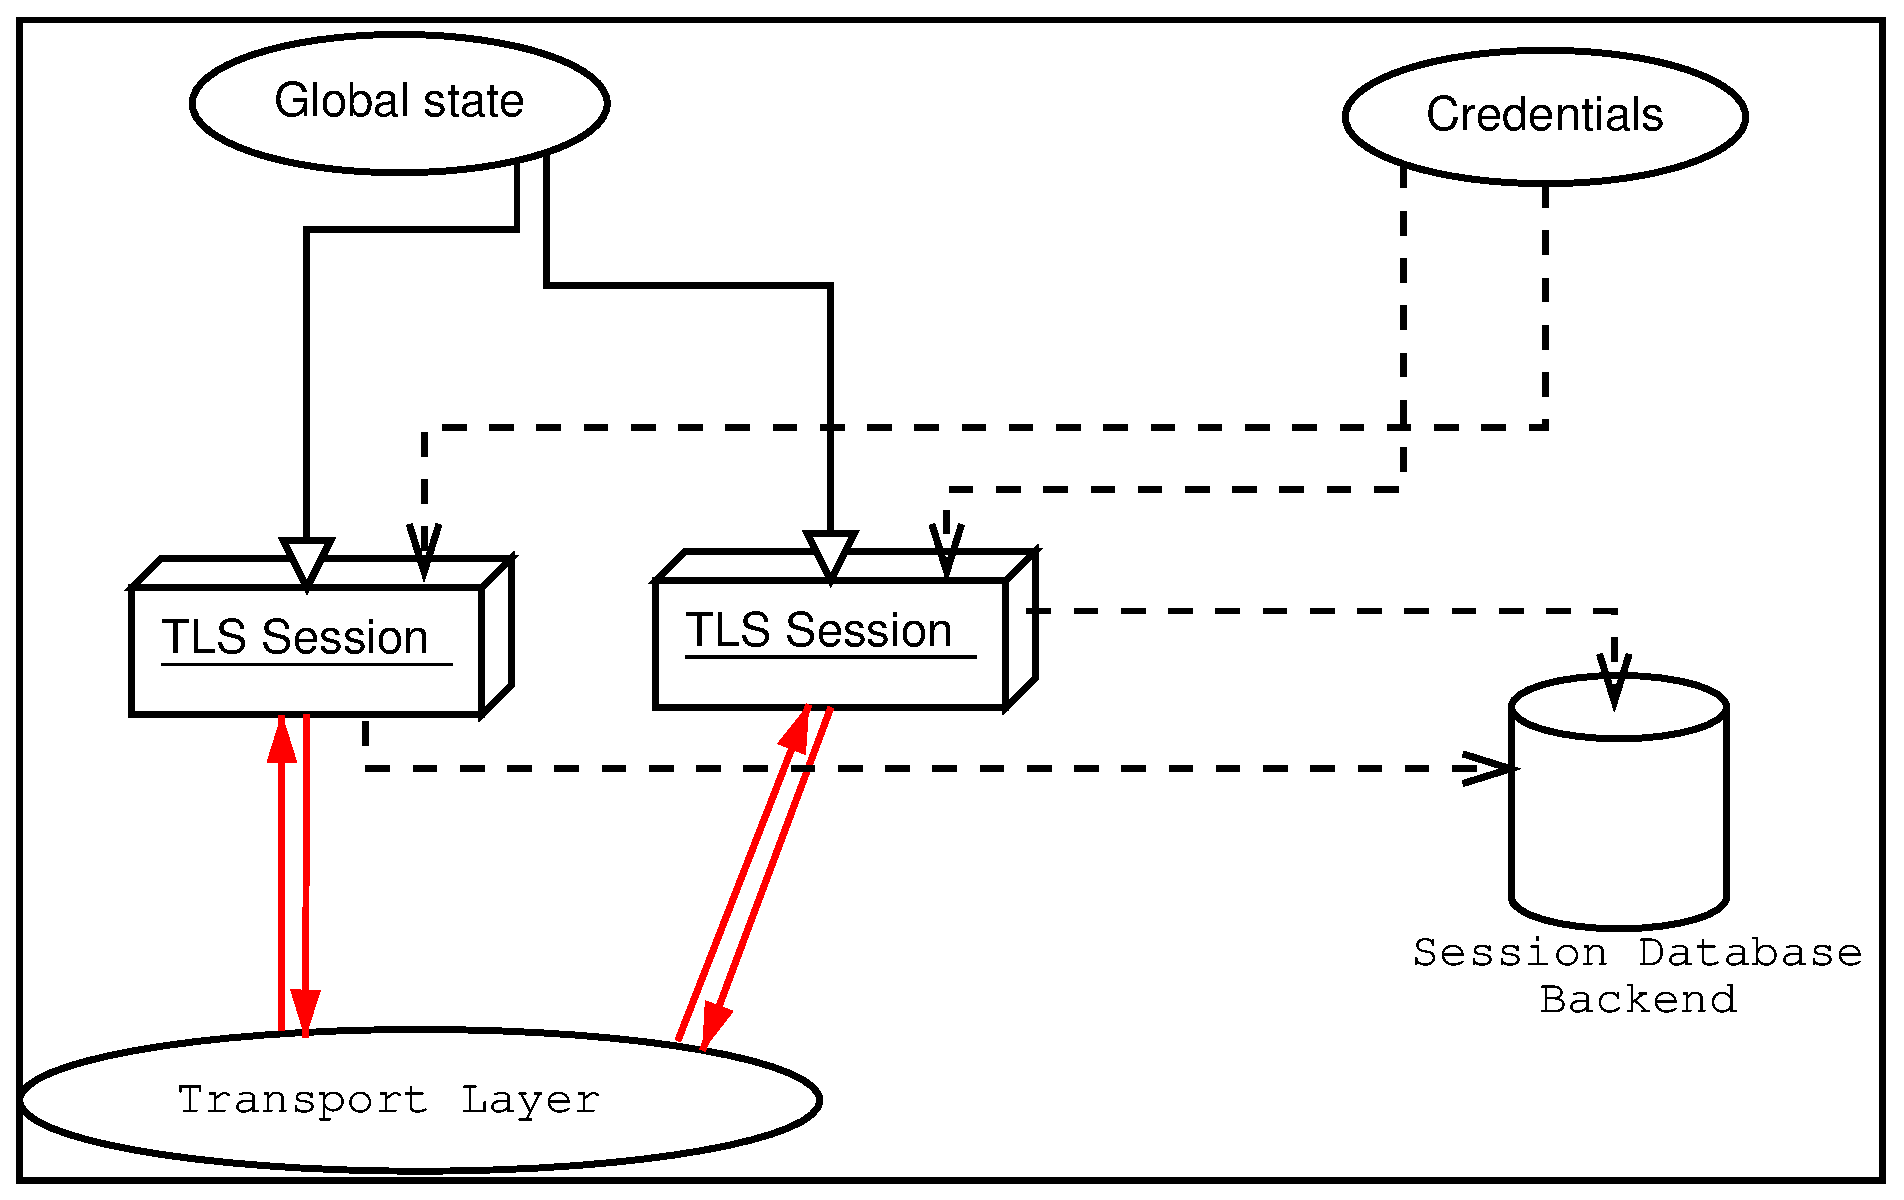
\includegraphics[height=8cm,width=12cm]{internals}
\label{fig:internals}
\end{figure}

\par
As shown in the figure, there is a read-only global state that
is initialized once by the global initialization function.
This global structure, among others, contains the memory allocation
functions used, and some structures needed for the ASN.1 parser.
This structure is never modified by any \gnutls{} function, except
for the deinitialization function which frees all memory allocated in
the global structure and is called after the program has permanently finished 
using \gnutls{}.

\par
The credentials structure is used within some authentication methods,
such as certificate authentication\footnote{see section \ref{certificate} on \pageref{certificate}}.
A credentials structure may contain certificates, private keys, temporary parameters 
for diffie hellman or RSA key exchange, and other stuff that may be shared
by several TLS sessions. 

This structure should be initialized using the appropriate initialization
functions. For example an application which uses certificate authentication
would probably initialize the credentials, using the appropriate functions,
and put it's trusted certificates in this structure. The next step is to
associate the credentials structure with each \tls{} session.

\par A \gnutls{} session contains all the required stuff for a
session to handle one secure connection. This session calls directly
to the transport layer functions, in order to communicate with the peer.
Every session has a unique session ID shared with the peer.

\par
Since TLS sessions can be resumed, servers would probably need a database
backend to hold the session's parameters. Every \gnutls{} session after
a successful handshake calls the appropriate backend function\footnote{see section \ref{resume}
on \pageref{resume} for information on initialization} to store the
newly negotiated session. The session database is examined by the server
just after having received the client hello\footnote{The first message
in a \tls{} handshake}, and if the session ID sent by the client,
matches a stored session, the stored session will be retrieved, and the
new session will be a resumed one, and will share the same session ID
with the previous one.

\section{Error handling\index{Error handling}}
\par
In \gnutls{} most functions return an integer type as a result.
In almost all cases a zero or a positive number means success, and
a negative number indicates failure, or a situation that some
action has to be taken. Thus negative error codes may be fatal
or not. 
\par 
Fatal errors terminate the connection immediately and
further sends and receives will be disallowed. An example of
a fatal error code is GNUTLS\_E\_DECRYPTION\_FAILED. Non-fatal errors
may warn about something, ie a warning alert was received, or
indicate the some action has to be taken. This is the case with
the error code GNUTLS\_E\_REHANDSHAKE returned by 
\printfunc{gnutls_record_recv}{gnutls\_record\_recv}.
This error code indicates that the server requests a re-handshake. The client
may ignore this request, or may reply with an alert.
You can test if an error code is a fatal one by using the
\printfunc{gnutls_error_is_fatal}{gnutls\_error\_is\_fatal}.
\par
If any non fatal errors, that require an action, are to be returned by a
function, these error codes will be documented
in the function's reference. All the error codes are documented
in appendix \ref{ap:error_codes} on page \pageref{ap:error_codes}.




\section{Memory handling}

\gnutls{} internally handles heap allocated objects differently, depending
on the sensitivity of the data they contain. However for performance
reasons, the default memory functions do not overwrite sensitive data from
memory, nor protect such objects from being written to the swap. 
In order to change the default behavior the
\printfunc{gnutls_global_set_mem_functions}{gnutls\_global\_set\_mem\_functions}
function is available which can be used to set other memory 
handlers than the defaults. 
\par
The \emph{libgcrypt} library on which \gnutls{} depends, has such secure
memory allocation functions available. These should be used in cases
where even the system's swap memory is not considered secure. See
the documentation of \emph{libgcrypt} for more information.



